\section{Aufbau}
\index{UMach!Aufbau}
\label{sec:Aufbau}

Die virtuelle UMach Maschine hat einen einfachen Aufbau, der im
wesentlichen aus den folgenden Komponenten besteht:
\begin{enumerate}
 \item Kern (Abschnitt \ref{sec:Kern})
 \item Speicher (Abschnitt \ref{sec:Speicher})
 \item I/O Einheit (Abschnitt \ref{sec:IO-Einheit})
\end{enumerate}

Siehe dazu Abbildung \ref{fig:umach-aufbau} auf Seite
\pageref{fig:umach-aufbau}.

\begin{figure}[htp]
 \centering
 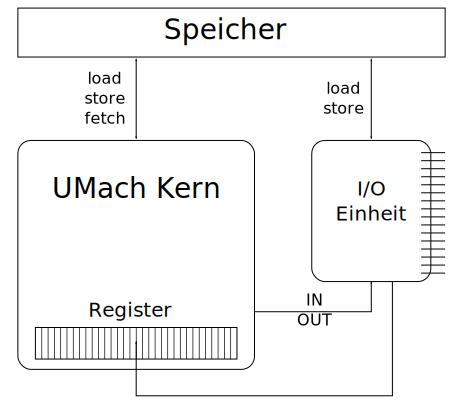
\includegraphics{./img/UMach-Aufbau.pdf}
 \caption{Aufbau der UMach Maschine}
 \label{fig:umach-aufbau}
\end{figure}

Beim Start der Maschine sucht diese nach einem ausführbaren Program im Speicher.
Bei Erfolg wird das gefundene Programm instruktionswise in den Kern geholt und
ausgeführt. Nach abarbeiten aller vorhandener Instruktionen verharrt die
Maschine in einem Wartezustand bis sie ausdrücklich ausgeschaltet wird.
Alle Eingabe- und Ausgabeoperationen werden an die I/O-Einheit weitergeleitet
und von dieser ausgeführt (siehe auch die Abschnitte \ref{sec:IO-Einheit} und
\ref{sec:IO-Instruktionen}).


\subsection{Betriebsmodi}
\label{subsec:Betriebsmodi}
\index{Betriebsmodus}

Die Umach VM kann in zwei verschiedenen Betriebsmodi oder auch
Betriebsarten betrieben werden:

\begin{enumerate}
  \item Normalmodus
  \item Debugmodus
\end{enumerate}

\paragraph{Normalmodus} Die virtuelle Maschine führt alle Instruktionen
ohne Unterbrechung aus. Nach der Ausführung schaltet sich die Maschine aus.

\paragraph{Debugmodus} Die virtuelle Maschine führt immer nur eine
einzige Instruktion aus und bleibt dannach stehen. Um mit der folgenden
Instruktion fortzufahren wird immer ein externen Signal benötigt.
Dieser Modus soll dem Entwickler erlauben, ein Programm schrittweise zu
debuggen.

Der Modus kann vor dem Hochfahren der Maschine festgelegt, jedoch im
Betrieb nicht mehr geändert werden. Wird kein Modus angegeben, startet die
Maschine im Normalmodus.




\subsection[Neumann Zyklus]{Von Neumann Zyklus}
\label{subsec:Neumann-Zyklus}

Der Von Neumann Zyklus der UMach ist auf 4 Schritte verkürzt. Dies ist möglich,
da die Instruktionsbreite immer aus 4 Wörtern besteht, und somit der 
\glqq\textsc{Fetch}\grqq\ von 
Befehl und zugehörigen Operanden in einem gemeinsamen Schritt durchgeführt
werden kann. Somit besteht der Zyklus aus einem beginnenden \textsc{Fetch}. Bei
diesem wird der an der im Programmcounter \texttt{PC} liegende Adresse
gespeicherte Befehl in das Instruktionsregister \texttt{IR} geladen. Danach
wird der im ersten Byte liegende Befehl mit Hilfe des Befehlsdecoders decodiert
und an der ALU entsprechend eingestellt. 

In einem dritten Schritt \textsc{Execute} wird die Instruktion ausgeführt. Der
theoretisch 4. Schritt, das Inkrementieren des Programmcounters PC, wird
parallel zu den \textsc{Fetch} und \textsc{Decode} Vorgängen ausgeführt. Diese
Tatsache ist bei Instruktionen, welche den Inhalt des PC manipulieren, zu
berücksichtigen. Siehe auch Abbildung \ref{fig:Neumann-Zyklus} auf der Seite
\pageref{fig:Neumann-Zyklus}.

Auflistung der Schritte:

\begin{enumerate}
 \item \textsc{Fetch} --
       Holen der Instruktion aus dem Speicher von der Adresse, welche im PC
       vorliegt.
 \item \textsc{Decode} --
       Decodieren des Befehles und Einstellen der ALU.
 \item \textsc{Execute} --
       Auführen des Befehles in der ALU.
 \item Update \texttt{PC} --
       Inkrementieren des \texttt{PC}. Findet parallel zu \textsc{Fetch} und
       \textsc{Decode} statt.
\end{enumerate}

\begin{figure}[h!tp]
 \centering
 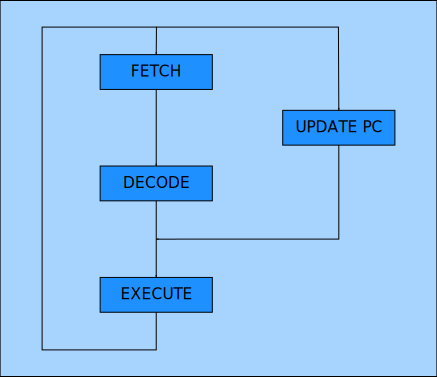
\includegraphics{./img/zyklus.pdf}
 \caption{Von Neumann Zyklus }
 \label{fig:Neumann-Zyklus}
\end{figure}


